% ---------------------------------------------------------------------------
% Preamble for the chemsim manual. Only packages that ship with the local
% MiKTeX install are used -- no on-the-fly downloads, which hang in a
% non-interactive shell.
% ---------------------------------------------------------------------------

\usepackage{framed}
\usepackage{tikz}
\usetikzlibrary{arrows.meta,positioning,calc,fit,backgrounds}
\usepackage{titlesec}
\usepackage{fancyhdr}
\usepackage{microtype}
% NO mathtools. Pandoc injects this file AFTER its own \usepackage{unicode-math},
% and mathtools loaded in that order silently destroys \underbrace and
% \overbrace -- they render as `|#{Z#}` tofu rather than as braces, with no
% "Missing character" warning anywhere in the log. Nothing here needs mathtools.

% ---- palette (matches the figures) ----------------------------------------
\definecolor{csblue}{HTML}{2A5C8A}
\definecolor{csred}{HTML}{B5442E}
\definecolor{csgreen}{HTML}{3F7A52}
\definecolor{csgold}{HTML}{C08A2E}
\definecolor{csgrey}{HTML}{5A5A5A}
\definecolor{csbluebg}{HTML}{EDF3F9}
\definecolor{csredbg}{HTML}{FBF0ED}
\definecolor{csgreenbg}{HTML}{EEF5F0}
\definecolor{csgoldbg}{HTML}{FCF6EA}
\definecolor{csrule}{HTML}{C8D2DC}

% ---- callouts: a coloured left rule plus a tint, breakable across pages ----
\makeatletter
\newenvironment{cs@bar}[2]{%
  \par\addvspace{9pt}%
  \def\FrameCommand{{\color{#2}\vrule width 2.6pt}\hspace{-1pt}%
    \colorbox{#1}}%
  \MakeFramed{\advance\hsize-\width \FrameRestore}%
}{\endMakeFramed\par\addvspace{9pt}}
\makeatother

\newenvironment{keypoint}[1][The point]%
  {\begin{cs@bar}{csbluebg}{csblue}%
   \noindent{\bfseries\color{csblue}\sffamily\footnotesize\MakeUppercase{#1}}\par\vspace{2pt}\noindent\ignorespaces}%
  {\end{cs@bar}}

\newenvironment{physics}[1][If you know physics]%
  {\begin{cs@bar}{csgreenbg}{csgreen}%
   \noindent{\bfseries\color{csgreen}\sffamily\footnotesize\MakeUppercase{#1}}\par\vspace{2pt}\noindent\ignorespaces}%
  {\end{cs@bar}}

\newenvironment{trap}[1][A trap this project actually fell into]%
  {\begin{cs@bar}{csredbg}{csred}%
   \noindent{\bfseries\color{csred}\sffamily\footnotesize\MakeUppercase{#1}}\par\vspace{2pt}\noindent\ignorespaces}%
  {\end{cs@bar}}

\newenvironment{aside}[1][Aside]%
  {\begin{cs@bar}{csgoldbg}{csgold}%
   \noindent{\bfseries\color{csgold}\sffamily\footnotesize\MakeUppercase{#1}}\par\vspace{2pt}\noindent\ignorespaces}%
  {\end{cs@bar}}

% ---- headings --------------------------------------------------------------
\titleformat{\chapter}[display]
  {\normalfont\sffamily\bfseries\color{csblue}}
  {\raggedright\normalsize\sffamily\color{csgrey}\MakeUppercase{\chaptertitlename\ \thechapter}}
  {6pt}
  {\Huge\raggedright}
  [\vspace{2pt}{\color{csrule}\titlerule[1.2pt]}]
\titlespacing*{\chapter}{0pt}{6pt}{22pt}

\titleformat{\section}
  {\normalfont\sffamily\large\bfseries\color{csblue}}{\thesection}{0.6em}{}
\titleformat{\subsection}
  {\normalfont\sffamily\normalsize\bfseries\color{csgrey}}{\thesubsection}{0.6em}{}

\titleformat{\part}[display]
  {\normalfont\sffamily\bfseries\color{csblue}\raggedright}
  {\Large\MakeUppercase{\partname\ \thepart}}
  {8pt}
  {\fontsize{30}{34}\selectfont\raggedright}

% ---- running heads ---------------------------------------------------------
\pagestyle{fancy}
\fancyhf{}
\renewcommand{\headrulewidth}{0.4pt}
\renewcommand{\headrule}{\hbox to\headwidth{\color{csrule}\leaders\hrule height \headrulewidth\hfill}}
% Only the chapter NUMBER on the left, so a long chapter title can never
% collide with a long section title on the right.
\renewcommand{\chaptermark}[1]{\markboth{\chaptername\ \thechapter}{}}
\renewcommand{\sectionmark}[1]{\markright{\thesection\quad #1}}
\fancyhead[L]{\footnotesize\sffamily\color{csgrey}\nouppercase{\leftmark}}
\fancyhead[R]{\footnotesize\sffamily\color{csgrey}\nouppercase{\rightmark}}
\fancyfoot[C]{\footnotesize\sffamily\color{csgrey}\thepage}
\fancypagestyle{plain}{\fancyhf{}\renewcommand{\headrulewidth}{0pt}%
  \fancyfoot[C]{\footnotesize\sffamily\color{csgrey}\thepage}}

% ---- table of contents -----------------------------------------------------
% The standard `report` \l@section reserves 2.3em for the number, which a
% double-digit subsection ("28.10") overruns straight into the title text.
% These are the stock definitions with wider number boxes.
\makeatletter
\renewcommand*\l@section{\@dottedtocline{1}{1.5em}{3.4em}}
\renewcommand*\l@subsection{\@dottedtocline{2}{4.9em}{4.2em}}
\makeatother

% ---- misc ------------------------------------------------------------------
\setlength{\emergencystretch}{4em}
\widowpenalty=10000
\clubpenalty=10000
\renewcommand{\arraystretch}{1.15}

% Shorthands used throughout the text.
\newcommand{\dd}{\mathrm{d}}
\newcommand{\std}{^{\circ}}
\newcommand{\smi}[1]{\texttt{\small #1}}

% ---- headroom for the running heads ---------------------------------------
\setlength{\headheight}{20pt}
\addtolength{\topmargin}{-8pt}

% ---- a title page worth the document ---------------------------------------
\renewcommand{\maketitle}{%
  \begin{titlepage}
  \thispagestyle{empty}
  \begin{tikzpicture}[remember picture,overlay]
    \fill[csblue] (current page.north west) rectangle
      ([yshift=-46mm]current page.north east);
    \node[anchor=north west,text width=125mm,inner sep=0pt]
      at ([shift={(32mm,-20mm)}]current page.north west)
      {\color{white}\sffamily\bfseries\fontsize{34}{38}\selectfont The chemsim Manual};
    \node[anchor=north west,text width=125mm,inner sep=0pt]
      at ([shift={(32mm,-33mm)}]current page.north west)
      {\color{white!85}\sffamily\fontsize{13}{16}\selectfont
       An emergent chemistry engine, explained from the beginning};
  \end{tikzpicture}
  \vspace*{58mm}\par
  {\sffamily\color{csgrey}\large
   A self-contained guide for a reader who knows physics\
   and has never done any chemistry.\par}
  \vspace{9mm}
  {\color{csrule}\rule{\textwidth}{1.2pt}}\par
  \vspace{5mm}
  {\sffamily\footnotesize\color{csgrey}
   Molecules are graphs. Reactions are graph-rewrite rules. Everything else ---
   yields, side products, boiling points, which product wins at which
   temperature --- is computed by integrating the system forward in time,
   rather than looked up.\par}
  \vfill
  \begin{tikzpicture}
    \foreach \y/\name/\what in {%
      7/{Layer 7}/{the window: a worker thread over the engine},
      6/{Layer 6}/{the headless stepper: events, waits, save and replay},
      5/{Layer 5}/{the vessel: four phases, pressure, energy balance},
      4/{Layer 4}/{the numeric core: stiff ODEs, activity, the Rust seam},
      3/{Layer 3}/{the network: discover reactions, derive reverse rates},
      2/{Layer 2}/{templates: SMARTS graph rewrites plus kinetics},
      1/{Layer 1}/{properties: thermochemistry, volatility, condensed phase},
      0/{Layer 0}/{matter: molecular graphs, canonical identity}}
    {
      \fill[csbluebg] (0,\y*0.62) rectangle (14.2,\y*0.62+0.54);
      \fill[csblue] (0,\y*0.62) rectangle (0.09,\y*0.62+0.54);
      \node[anchor=west,font=\sffamily\bfseries\scriptsize,text=csblue]
        at (0.35,\y*0.62+0.27) {\name};
      \node[anchor=west,font=\sffamily\scriptsize,text=csgrey]
        at (2.2,\y*0.62+0.27) {\what};
    }
  \end{tikzpicture}
  \vspace{8mm}\par
  {\sffamily\footnotesize\color{csgrey}
   Generated from the \texttt{chemsim} repository \quad\textbullet\quad 29 August 2026\par}
  \end{titlepage}
}
